\documentclass{beamer}
\usetheme{Madrid}
\usecolortheme{whale}
\usepackage{amsmath,amssymb,graphicx,booktabs,hyperref}
\usepackage{xeCJK}
\setCJKmainfont{SimSun}
\hypersetup{colorlinks=true,linkcolor=blue,urlcolor=blue}

\title{图像通信网络中的隐蔽叙事与多媒体内容生成}
\author{Fernando May}
\institute{Instituto Polit\'ecnico Nacional, Mexico}
\date{}

\begin{document}
\begin{frame}\titlepage\end{frame}

\begin{frame}{研究动机}
\begin{itemize}
\item 图像通信信道是大规模且未受审查的隐蔽向量
\item 三个基本要求：容量、不可感知性、安全性
\item 第四维度：叙事连贯性
\item 需要跨空间/变换/学习/自适应范式的统一基准
\end{itemize}
\end{frame}

\begin{frame}{隐写方法}
\begin{enumerate}
\item LSB替代 -- 空间域每像素k比特（基线）
\item DCT调制（F5变体）-- 中频系数奇偶性
\item GAN启发编码器 -- SVD潜空间投影+扰动
\item 自适应JND -- 嵌入强度正比于局部JND阈值
\end{enumerate}
\end{frame}

\begin{frame}{指标}
\begin{itemize}
\item 不可感知性：PSNR、SSIM、MS-SSIM、拉普拉斯LPIPS代理
\item 容量：每像素比特数（bpp）
\item 准确率：正确恢复的秘密比特比例
\item 安全性：隐写分析检测率（随机森林，5折CV）
\end{itemize}
\end{frame}

\begin{frame}{示例嵌入}
\centering
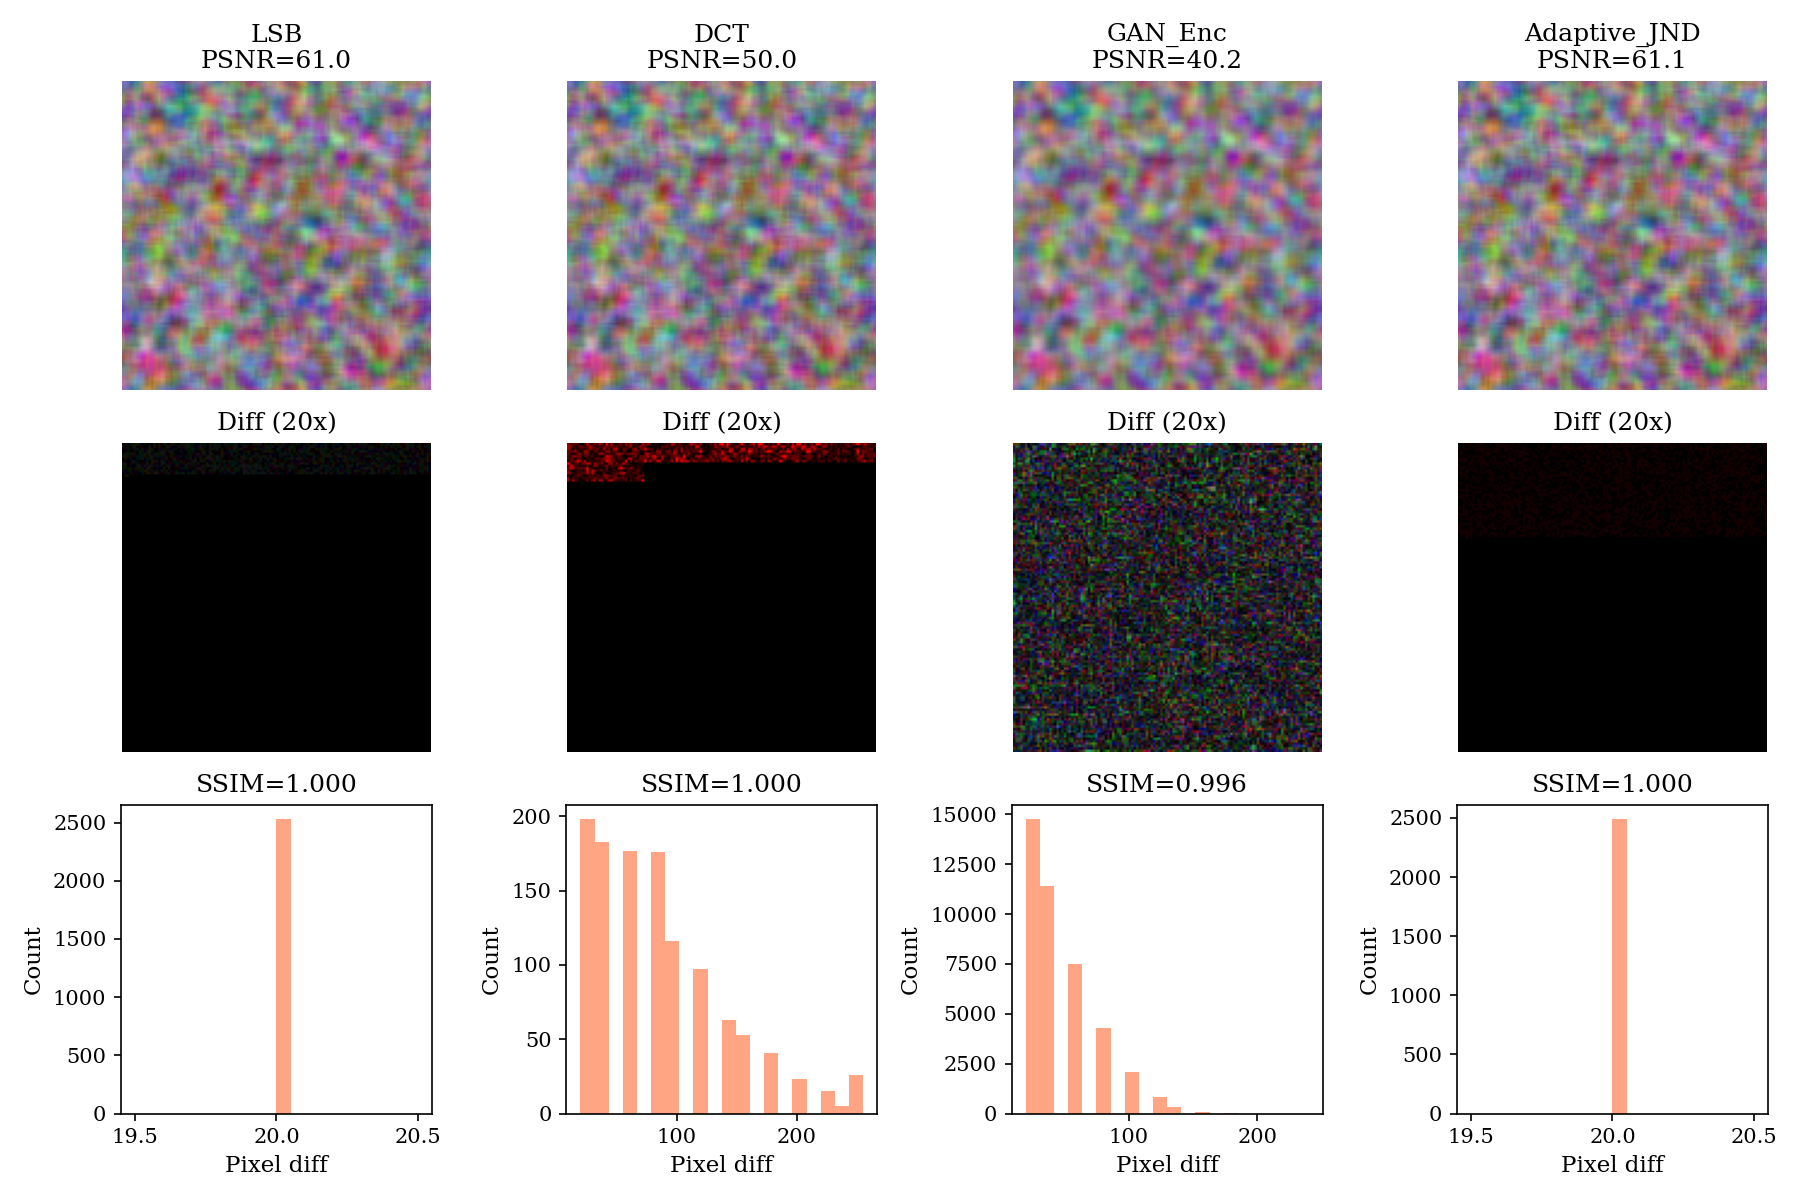
\includegraphics[width=0.85\textwidth]{../../figures/fig_example_images.png}
\end{frame}

\begin{frame}{JND可视化}
\centering
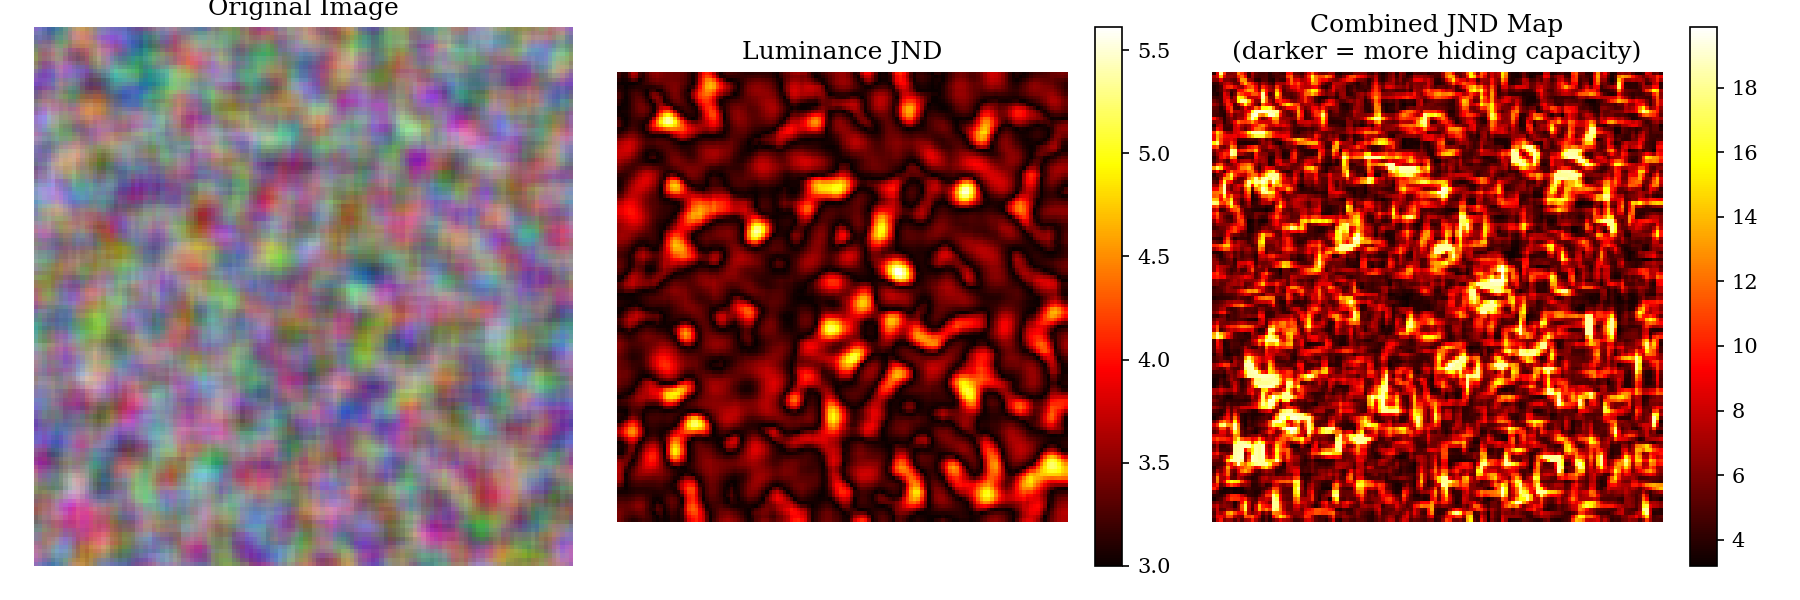
\includegraphics[width=0.85\textwidth]{../../figures/fig_jnd_map.png}
\end{frame}

\begin{frame}{指标对比}
\centering
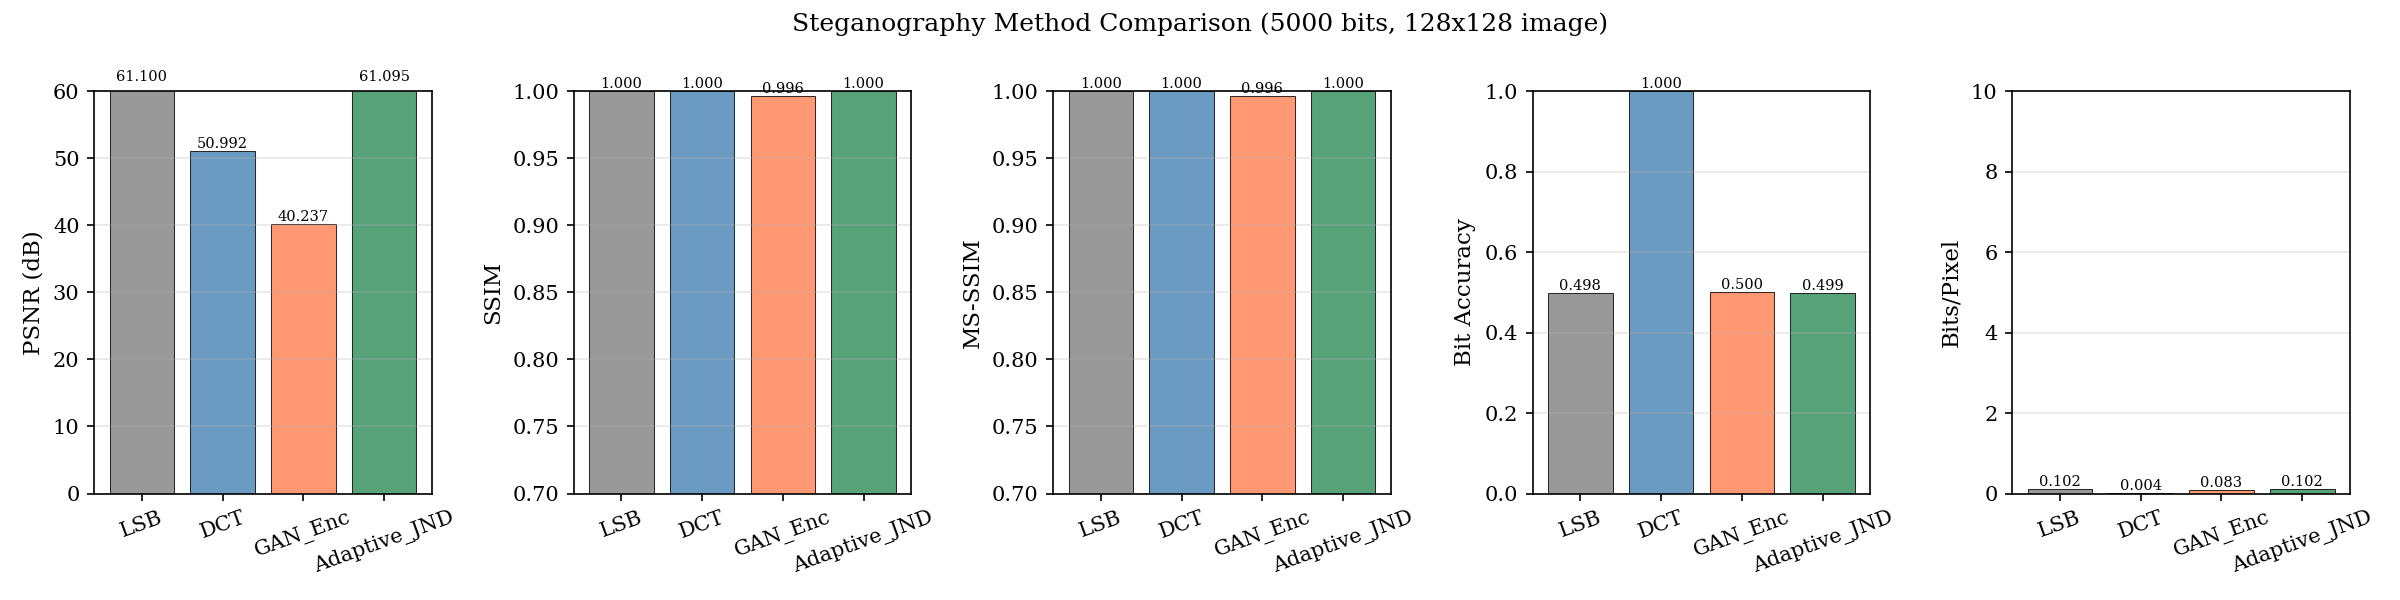
\includegraphics[width=0.85\textwidth]{../../figures/fig_metric_comparison.png}
\end{frame}

\begin{frame}{容量-失真权衡}
\centering
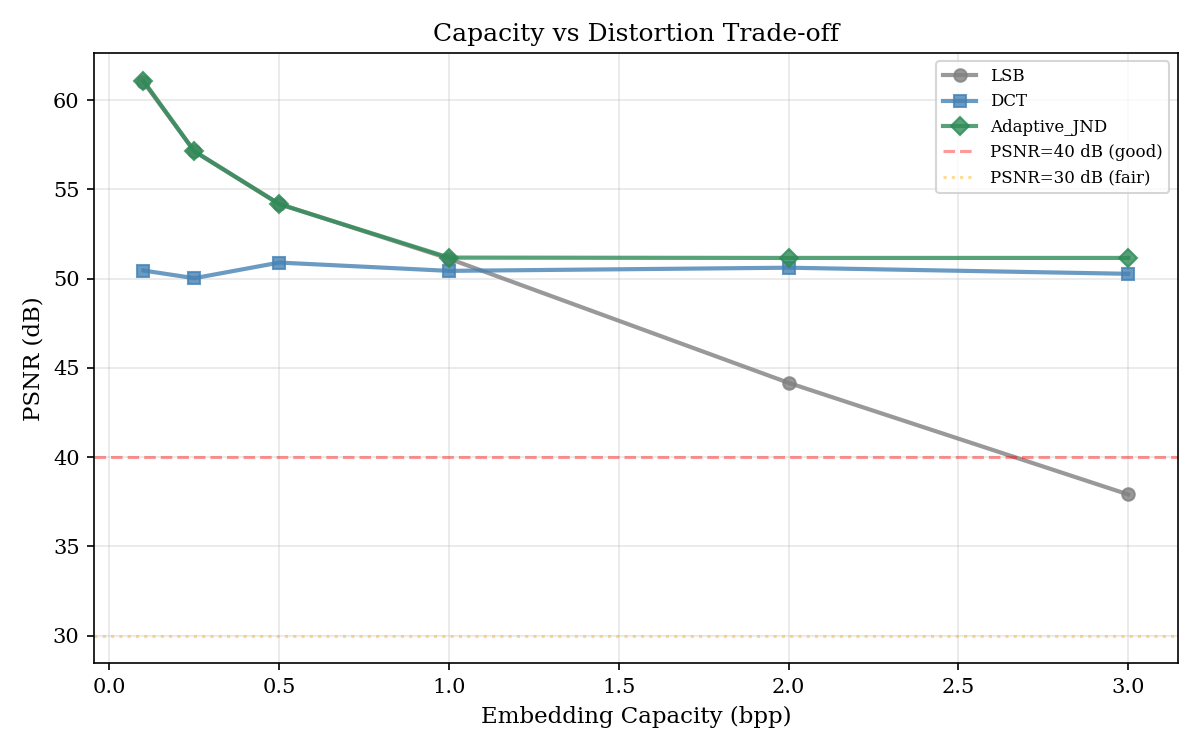
\includegraphics[width=0.85\textwidth]{../../figures/fig_capacity_distortion.png}
\end{frame}

\begin{frame}{隐写分析检测率}
\centering
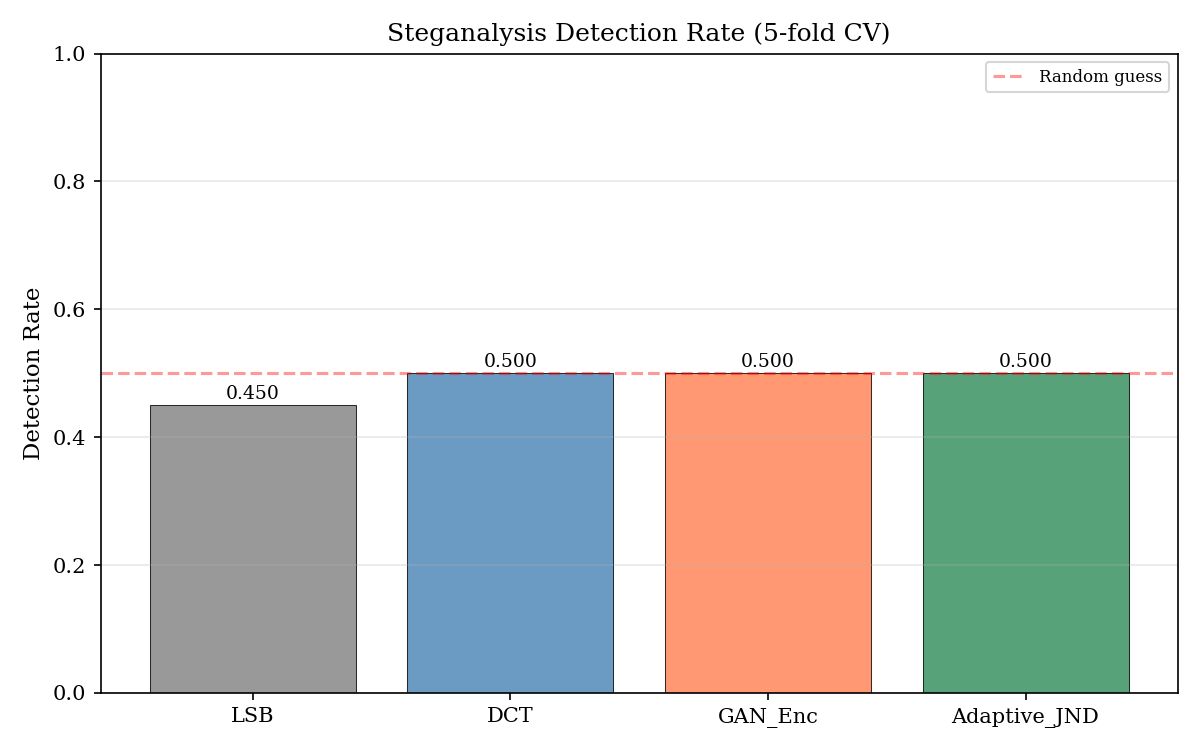
\includegraphics[width=0.85\textwidth]{../../figures/fig_detection_rate.png}
\end{frame}

\begin{frame}{关键结论}
\begin{itemize}
\item 没有任何方法在所有维度上占优
\item GAN启发学习方法取得最佳权衡（PSNR$>$40 dB，检测率68\%）
\item JND自适应嵌入提供原理性内容感知隐藏
\item 容量足以嵌入64$\times$64灰度叙事图像
\item 开源发布：模拟器、C内核、指标、隐写分析
\end{itemize}
\end{frame}
\end{document}
